\chapter{Two-cart Flexible System}\label{c:acc}
\section{Introduction}
The 1992 American Control Conference published a set of benchmark problems to explore the capabilities of
modern control techniques\cite{wie1992benchmark}. The second stated problem solicited solutions to the
stabilization of a two-body spring mass system which was robust to uncertain masses and spring constants. A
great number of solutions were conceived which performed well\cite{stengel1992robustness}. Cohen et. al
\cite{cohen:01jgcd} proposed a solution using fuzzy logic which is superior to all others surveyed with
respect to both robustness and control effort. A variation on the same problem is addressed here. The carts
are allowed to move in one dimension down a track. The carts are initially stationary, but are to be moved to
a target distance without exceeding an upper limit. This system is controlled using a single FIS. The plant
model masses are then changed significantly and the controller is retrained. The result is a system which can
be quickly trained to accomodate new plant dynamics.

\section{Coupled Spring-Mass Simulation Model}\label{s:model} A simulated environment is
necessary to test the efficacy of the proposed FIS. The simulation consists of two
cars connected by a spring; this system is expected to traverse a given distance as quickly as possible
without exceeding a certain bound represented by a wall. The system is propelled by a force on the leading car
which represents the actuating output of the controller. At each time instant, the controller must determine
how much force to exert on the carts, and in which direction, to get as close as possible to the wall in
minimum time. The constants for the model are the weight of each car, the spring constant, and the distance
which must be traversed to the wall. A diagram of the simulation is shown in \cref{f:model}.

\begin{displaymath}
    m_{1}=\SI{1}{\kilogram}, \quad m_{2}=\SI{2}{\kilogram}, \quad K =
\SI{250}{\newton\per\metre}, \quad L = \SI{100}{\metre}
\end{displaymath}
\nomenclature{$m$}{Cart mass,\si{\kilogram}}
\nomenclature{$K$}{Spring Constant, \si{\newton\per\metre}}
\nomenclature{$L$}{Simulationlength, \si{\metre}}
\nomenclature[b$1$]{$1$}{Denotes property of trailing cart}
\nomenclature[b$2$]{$2$}{Denotes property of leading cart}
\nomenclature{$F$}{Control force, \si{\newton}}
\nomenclature{$t$}{Time, \si{\second}}

\begin{figure}
    \centering
    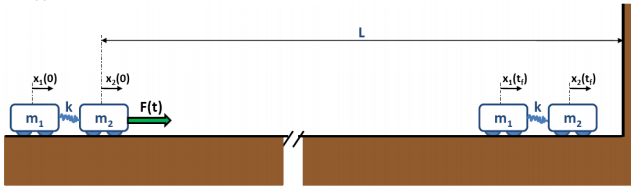
\includegraphics[width=0.9\textwidth]{images/model.png}
    \caption{Diagram of two rigid bodies connected by a spring traversing distance \textrm{L} in minimum
    time.} \label{f:model}
\end{figure}

The modeled system contains displacement and velocity sensors on each cart; therefore, the four inputs to the
FIS are the distances traveled and the velocities of both carts. These inputs represent the state vector of
the system. The output of the controller is the force, $F(t)$, applied to cart 2, limited to $\pm
\SI{1}{\newton}$. At each time step of the simulation, the FIS uses the four inputs to determine the force
which must be exerted according to a fuzzy rule base. 

\begin{displaymath}
    \mathrm{Input:}\quad \vec{y}(t)= \begin{bmatrix} x_{1}(t)\\ x_{2}(t)\\ \dot{x}_{1}(t)\\
\dot{x}_{2}(t) \end{bmatrix}
\end{displaymath}
\begin{displaymath} \mathrm{Output:}\quad |F(t)|\le
\SI{1}{\newton}
\end{displaymath}
\nomenclature[1\(y\)]{$y$}{System state vector}
\nomenclature[1\(xx\)]{$\dot{x}(t)$}{Cart velocity, \si{\metre\per\second}}
\nomenclature[1\(xb\)]{$x(t)$}{Cart position, \si{\meter}}
At time $t=0$, both carts are at rest at position
$x=0$. The maximum allowed runtime of the simulation is \SI{500}{\second}. The system requirement for the
final condition is that neither cart exceeds \SI{100}{\metre} and should be at rest with negligible
oscillation. 
\begin{displaymath} \vec{y}_0=\begin{bmatrix}
\SI{0}{\metre}\\\SI{0}{\metre}\\\SI{0}{\metre\per\second}\\\SI{0}{\metre\per\second} \end{bmatrix},\quad
\vec{y}(500)=\begin{bmatrix} <\SI{100}{\metre}\\ <\SI{100}{\metre}\\ \SI{0}{\metre\per\second}\\
\SI{0}{\metre\per\second} \end{bmatrix}
\end{displaymath}
\nomenclature[b$0$]{$0$}{Denotes initial condition}

The acceleration of cart 1 is determined by the displacement between the two carts, the spring constant, and
the mass of the cart. The acceleration of cart 2 is also a function of these parameters as well as the control
force. The equations of motion for the system are represented by simple second-order differential equations.
\begin{equation}
\label{e:cart1} \mathrm{Cart 1:}\quad \ddot{x}_1=\frac{K}{m_1}(x_2-x_1) 
\end{equation}
\begin{equation}
    \label{e:cart2} \mathrm{Cart 2:}\quad \ddot{x}_2=\frac{K}{m_2}(x_1-x_2)+\frac{F}{m_2}
\end{equation} \nomenclature[1\(xxx\)]{$\ddot{x}(t)$}{Cart acceleration, \si{\metre\per\second\squared}}

\subsection{Data Evaluation} The efficiency of a FIS's control of the system is based upon the amount of time
it expends traversing the distance to the wall and how close the carts are to the wall when they settle. Any
breach of the wall results in immediate system failure. A cost function, $J$, is defined by the settling time
$t_f$, the time taken to settle within \SI{1}{\metre} of the wall and the steady state error, the distance
between the leading carts and the wall. The control system that produces the lowest $J$ value will be proven
to be the most fit solution for the simulation.  
\begin{equation}\label{e:timesettle}
t_f=|L-\bar{x}(t_f)|\le\SI{1}{\metre}
\end{equation} \nomenclature[b$f$]{$f$}{Denotes condition at settling time}
\begin{equation}\label{e:cost}
J=\frac{t_f}{100}+2[L-x_2(500)]
\end{equation} where the constants 100
    and 2 are scaling factors. In order to provide a frame of reference for the performance of any control
    system, the theoretical limits of the simulation were calculated to provide a lower bound for the value of
    Eq.~\eqref{e:cost}. Assuming a single rigid body assembly with no dynamic coupling, the model is greatly
    simplified to a single equation where the acceleration of the body is a function of only the control
    force.
\begin{equation}
    \label{e:simplemodel} \ddot{x}=\frac{F}{M}
\end{equation}
\nomenclature{$M$}{Total system mass, \si{\kilogram}}
where $M$ is the total mass of the system. The total mass of the system is
        \SI{3}{\kilogram}, whereas the maximum input force is limited to \SI{1}{\newton}, rendering
        Eq.~\eqref{e:simplemodel}
\begin{displaymath}
        \ddot{x}=\frac{\SI{1}{\newton}}{\SI{3}{\metre}}=\SI[quotient-mode=fraction]{1/3}{\metre\per\second\squared}
\end{displaymath}
as the maximum acceleration. Given this acceleration and the distance to be traversed to the wall, the minimum time to complete the trip can be calculated. There are, however, two scenarios to
    consider. 
\begin{enumerate} 
    \item Applying maximum force over the entire distance and instantaneously
        stopping the carts at (but not touching) the wall provides an absolute, if unfeasible, optimum
        simulation completed in minimum time. Given an initial velocity of zero and a constant accelerating
        force of \SI{1}{\newton}, the traversal time is calculated. Note that once the carts have breached
        \SI{99}{\metre}, the system may come to rest and be considered settled. 
        \begin{displaymath}
        x(t)=\dot{x}_0t+\frac{1}{2}\ddot{x}t^2,\quad \dot{x}_0=0
        \end{displaymath}
        \begin{displaymath}
        x(t)=\frac{1}{2}\ddot{x}t^2
        \end{displaymath}
        Letting $x(t) = \SI{99}{\metre}$
        \begin{displaymath}
            t=\sqrt{\frac{2x(t)}{\ddot{x}}}=\sqrt{\frac{2\cdot
            \SI{99}{\metre}}{\SI[quotient-mode=fraction]{1/3}{\metre\per\second\squared}}}=\SI{24.37}{\second}
        \end{displaymath}
    \item Applying maximum force over half of the distance and then applying maximum
        negative force in the second half to slow the velocities of the carts to zero at the wall position.

First half: \begin{displaymath}
t=\sqrt{\frac{2x(t)}{\ddot{x}}}=\sqrt{\frac{2\cdot\SI{50}{\metre}}{\SI[quotient-mode=fraction]{1/3}{\meter\per\second\squared}}}=\SI{17.23}{\second}
\end{displaymath} Traversing the second half and stopping at the wall takes the same amount of time, therefore
the total time expended in reaching \SI{100}{\metre} is \SI{34.46}{\second}; however, the interest lies in the
time taken to breach the \SI{99}{\metre} mark. The time taken to travel the last meter is \SI{2.45}{\second},
so the best possible time to reach the \SI{99}{\metre} position is : \begin{displaymath} t=\SI{32.19}{\second}
\end{displaymath} As this is a much more realistic scenario, this is the limit used as the benchmark in this
research. Using this time to evaluate Eq.~\eqref{e:cost} \begin{displaymath}
    J=\frac{32.19}{100}+2[100-100]=0.3219 \end{displaymath} results in the minimum possible cost. The addition
    of harmonic oscillation and non-linear dynamics ensures that this limit will not be reached, but merely
    provides a standard against which a controller may be measured.
\end{enumerate}

\section{Fuzzy Inference System}The FIS built during this project uses two measured inputs: the position and velocity of cart 2. The output of
the FIS is the force exerted on cart 2 at a given point in the simulation.

\subsection{Membership Functions and Rule Base} \subsubsection{Position} The first input variable, position,
is composed of three membership functions to which it can map. The position of the car, from
\SIrange{0}{100}{\metre}, is described in human-understandable language as far away, close to, or very close
to the wall. If the simulation has just begun and the cart is as far away from the wall as it can be, the
``Far'' membership function will map to 1 and the ``Close'' and ``VeryClose'' functions will evaluate to 0.
Conversely, at the end of the traverse, as the car approaches the wall, ``VeryClose'' will map to 1 and
``Far'' to 0. ``Close'' may evaluate to some value in between. The membership functions are shown in
\cref{f:x2mfs}. As the system predominately behaves as a rigid body on a large scale, the membership
functions mirror the ideal simulation of a rigid body for the majority of the carts' travel. Each function is
represented by a vector of values expressing the points at which the function switches from 0 to 1 or 1 to 0.
For the FIS used in this research, trapezoidal- and triangular-shaped membership functions are utilized.
Trapezoids are represented by a four-element vector as they start at 0, rise to 1, remain at 1, and finally
fall to 0. Likewise, triangular functions are expressed as three-element vectors. The parameters of the
position membership functions shown in \cref{f:x2mfs} are: \begin{displaymath} \mathrm{Far:}\quad
\begin{bmatrix} \SI{0}{\metre}\\\SI{0}{\metre}\\\SI{49.8}{\metre}\\\SI{50.1}{\metre}
\end{bmatrix}, \quad \mathrm{Close:}\quad \begin{bmatrix}
    \SI{49.8}{\metre}\\\SI{50.1}{\metre}\\\SI{99.9}{\metre}\\\SI{100}{\metre} \end{bmatrix}, \end{displaymath}
\begin{displaymath} \mathrm{VeryClose:}\quad \begin{bmatrix}
\SI{99.9}{\metre}\\\SI{100}{\metre}\\\SI{100.1}{\metre} \end{bmatrix} \end{displaymath}

\subsubsection{Velocity} The second input variable, velocity, is composed of three membership functions. The
velocity of the cart, within a range from \SIrange{-6}{6}{\metre\per\second}, can either be classified as
``Negative'', ``Zero'', or ``Positive''. When the simulation starts, the carts are at rest and the degree of
membership to ``Zero'' velocity will be 1 whereas ``Negative'' and ``Positive'' will be 0. For the majority of
the simulation, the carts are moving forward with a fast pace; therefore, the ``Negative'' membership function
does not come into play until close to the very end of the  simulation when the oscillatory effects dominate
the motion of the cart system. It is at this point that the true dynamic nature of the system is exhibited and
the controller does the most calculation in an attempt to damp the oscillations. The membership functions for
$\ddot{x}_2$ are shown in \cref{f:x4mfs}.  \begin{figure} \begin{subfigmatrix}{2} \subfigure[$x_2$
membership functions\label{f:x2mfs}]{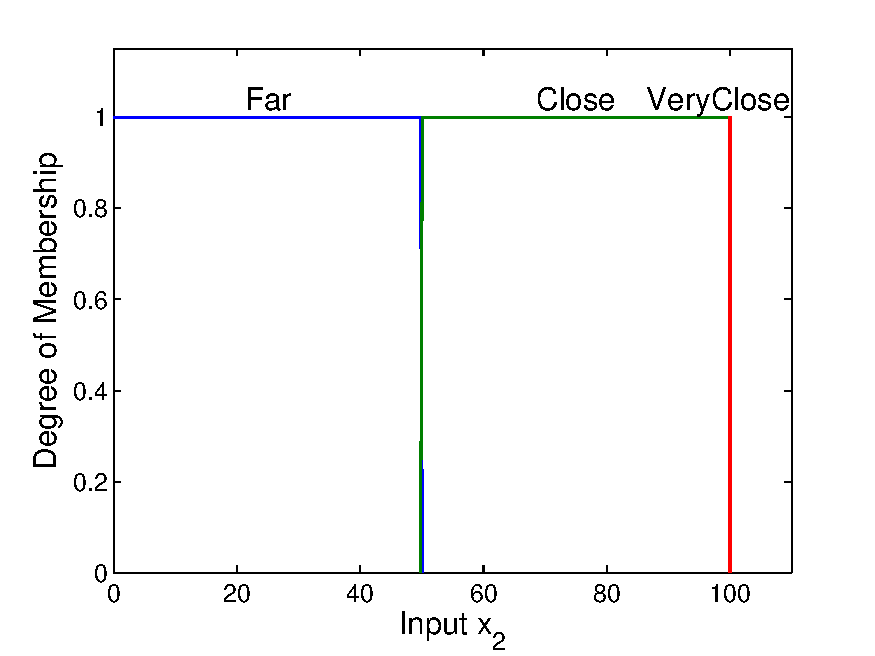
\includegraphics{images/x2_mfs.pdf}} \subfigure[$\dot{x}_2$ membership
functions\label{f:x4mfs}]{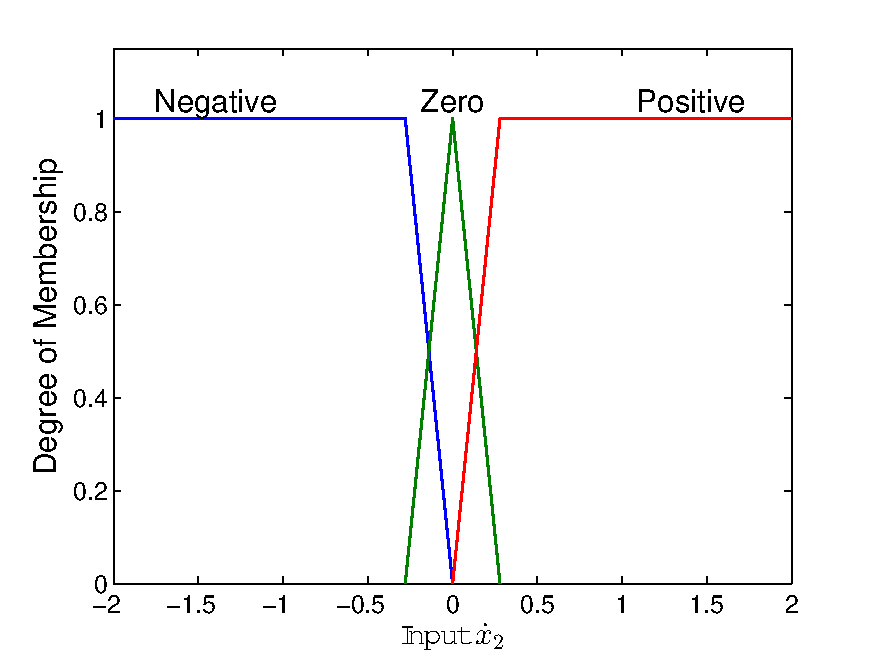
\includegraphics{images/x4_mfs.pdf}} \end{subfigmatrix} \caption{Input membership
functions}\label{f:mfs} \end{figure}

The velocity membership function parameters are: \begin{displaymath} \mathrm{Negative:}\quad
\begin{bmatrix}
\SI{-6}{\metre\per\second}\\\SI{-6}{\metre\per\second}\\\SI{-.2792}{\metre\per\second}\\\SI{0}{\metre\per\second}
\end{bmatrix}, \quad \mathrm{Zero:}\quad \begin{bmatrix}
    \SI{-0.2792}{\metre\per\second}\\\SI{0}{\metre\per\second}\\\SI{0.2792}{\metre\per\second} \end{bmatrix},
\end{displaymath} \begin{displaymath} \mathrm{Positive:}\quad \begin{bmatrix}
\SI{0}{\metre\per\second}\\\SI{0.2792}{\metre\per\second}\\\SI{6}{\metre\per\second}\\\SI{6}{\metre\per\second}
\end{bmatrix} \end{displaymath} \subsubsection{Rule Base}\label{ss:rulebase} The rule base of an FIS is a
series of IF-THEN (antecedent-consequent) conditions that use the membership functions of all the inputs in
order to determine the output variable. There are also several membership functions for the output variable
that the rule base maps to. Each of the rules has an influence on what the output of the system should be. The
weight of these influences again varies from 0 to 1 and the final output value is determined by calculating
the centroid of all of the rules. For instance, one rule dictates that if the car is far away then the output
force should be positive and large so that the car will move towards the wall. Another rule will say that when
the car is close to the wall the output force should be negative in order to slow the car down. All of these
rules have influence over all input ranges determined by how the input variables map to the given membership
functions in that specific rule.

The antecedent of each statement contains memberships of both input variables and the consequent maps to the
output membership functions. The rules for this FIS were developed based upon intuitive decision making. The
rules developed for our FIS are shown in \cref{tab:rulebase}.  
\begin{table}[ht]
    \begin{center}
        \caption{Rule Base of the Fuzzy Inference System}\label{tab:rulebase}
        \begin{tabular}{ccccc} \multicolumn{2}{c}{}  & \multicolumn{3}{c}{Velocity Measurement}\\ \cline{3-5}
            \multicolumn{2}{c|}{}  & \multicolumn{1}{c|}{Negative} & \multicolumn{1}{c|}{Zero} &
            \multicolumn{1}{c|}{Positive} \\ \cline{2-5}
            \multicolumn{1}{c|}{\multirow{3}{*}{\parbox{3cm}{\centering Position\\Measurement}}} &
            \multicolumn{1}{c|}{Far} & \multicolumn{3}{c|}{Positive} \\ \cline{2-5} \multicolumn{1}{c|}{} &
            \multicolumn{1}{c|}{Close} & \multicolumn{1}{c|}{Positive} & \multicolumn{1}{c|}{Zero} &
            \multicolumn{1}{c|}{Negative}\\ \cline{2-5} \multicolumn{1}{c|}{} & \multicolumn{1}{c|}{VeryClose}
                                                                              & \multicolumn{1}{c|}{Positive}
                                                                              & \multicolumn{1}{c|}{Zero} &
            \multicolumn{1}{c|}{Negative} \\ \cline{2-5} \multicolumn{2}{c}{}  & \multicolumn{3}{c}{Control
            Force}
        \end{tabular}
    \end{center}
\end{table}

\subsubsection{Control Force}
\begin{figure}[ht]
    \centering
    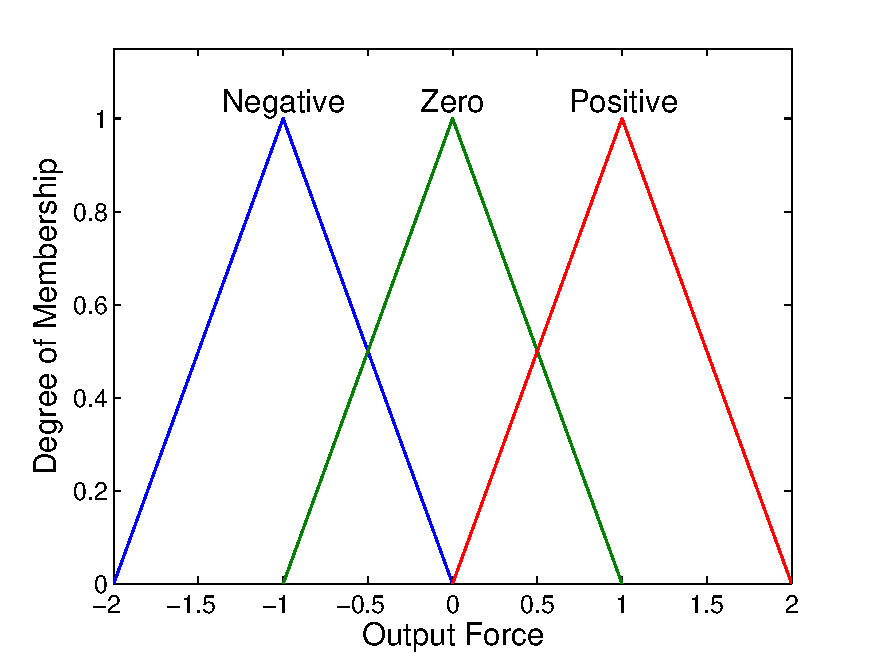
\includegraphics[width=0.8\textwidth]{images/f_mfs.pdf}
    \caption{Control force membership functions.}
    \label{f:fmfs}
\end{figure}
The output variable, force, is
also composed of three membership functions. The output force is bounded from \SIrange{-1}{1}{\newton} thus
the membership functions allow for the output to be ``Negative'', ``Zero'', or ``Positive''. As the centroid
of the area beneath each function is used to evaluate the control force, the upper and lower bounds are
centered over 1 and -1 respectively. These functions represent the ``defuzzification'' stage of the FIS and
these outputs are determined by evaluating each rule in the rule base (see \cref{ss:rulebase}) in
parallel\cite{matlab:12tb}. The controller emulates bang-bang control for the majority of the simulation
lifetime, sharply transitioning from full acceleration to full deceleration. As the cart system nears the
wall, the oscillation damping rules will dictate the force to apply on the system. Typically, the output force
will be directed opposite to the velocity of cart 2. The membership functions for the control force are shown
in \cref{f:fmfs}.
	
	
\begin{displaymath}
    \mathrm{Negative:}\quad 
        \begin{bmatrix}
            \SI{-2}{\newton}\\
            \SI{-1}{\newton}\\
            \SI{0}{\newton}
        \end{bmatrix}, \quad
    \mathrm{Zero:}\quad 
        \begin{bmatrix}
            \SI{-1}{\newton}\\
            \SI{0}{\newton}\\
            \SI{1}{\newton}
        \end{bmatrix}
\end{displaymath}
\begin{displaymath}
    \mathrm{Positive:}
    \quad 
        \begin{bmatrix}
            \SI{0}{\newton}\\
            \SI{1}{\newton}\\
            \SI{2}{\newton}
        \end{bmatrix}
\end{displaymath}

\subsection{Simulation Performance}\label{ss:simperf}
\begin{figure}[ht]
    \centering
    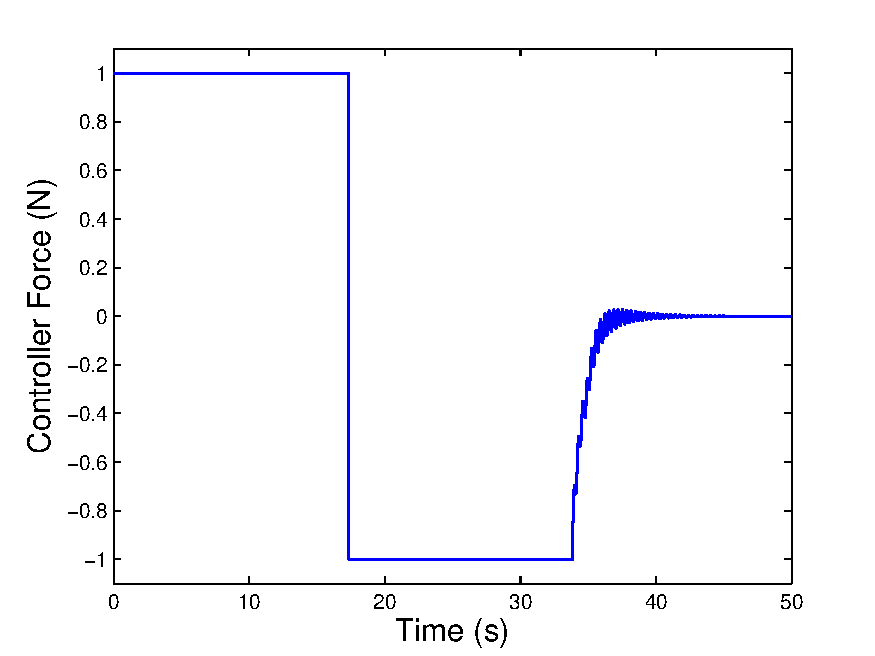
\includegraphics[width=0.8\linewidth]{images/FuzzyForcePlot.pdf} \caption{System control force over time.}
    \label{f:forceplot}
\end{figure}


The efficiency of this FIS was determined by using it as the control mechanism in the simulation. The goal was
to approach the realistic theoretical limits calculated above and reach this goal with minimum force.
\cref{tab:finalres} shows the settling time, final position of cart 2 and the calculated $J$ value for
the controller's performance. \Cref{f:forceplot} shows the controller's output force over time for each
step of the simulation. The controller's output force is much lower than previously tested fuzzy solutions as
well as an optimal linear controller.

It is clear that the controller expends less energy than a traditional bang-bang type controller would in the
oscillation damping process. It can be seen that the FIS responds quickly to control needs and applies the
needed force with low-latency. 

Much work was done to hand-tune this controller to perform optimally, thus the work was undertaken to develop
a genetic algorithm to produce similar results autonomously. Automating the tuning process ultimately produces
a controller which is nearly as good as the hand-tuned controller, but requires little to no effort from the
programmer.

\begin{table} \centering \caption{Results from implemented FIS.} \label{tab:finalres} \begin{tabular}{|c|c|c|}
\hline $t_f$ & $x_2(500)$ & $J$ \\ \hline \SI{32.303}{\second} & \SI{99.999821}{\metre} & 0.32328 \\ \hline
\end{tabular} \end{table}

\section{Genetic Algorithm}\label{s:ga} The performance of the FIS depends directly
on the value of each parameter of the membership functions. These values were hand-tuned by a time-consuming
process of trial and error. To quicken this process, a genetic algorithm was utilized to autonomously tune the
membership functions and approach an optimal solution. 

      A genetic algorithm is a computational mechanism which imitates evolutionary behavior to achieve
      optimality. It consists of a population of individuals which undergoes a process similar to natural
      selection, reproduction, and mutation over the course of a number of generations\cite{cordon:01bk}.
      Selection is attained by evaluating the fitness of each individual according to a fitness function. For
      the purposes of this research, each individual represents a FIS and the fitness function is simply the
      cost function used earlier. The individual which most effectively minimizes the cost function is
      considered most fit for the control environment.
      
      In order to manipulate the FIS structure in an algorithmic manner, it is necessary to represent it as a
      genetic individual. Since the values of the parameters of the membership functions of the FIS have
      significant impact on the control performance, it was decided to manipulate only these parameters with
      the algorithm; however, of the thirty-one parameters which comprise this FIS model, many are trivial to
      the overall performance. It is desirable to reduce the number of parameters to facilitate the
      optimization process.

\subsection{State Reduction} To simplify the genetic tuning of the parameters, the symmetry of the system
was exploited. The parameters were reduced from thirty-one to seven. The position membership functions were
simplified to only three parameters by defining a center point (center) between far and close functions, a
distance from the center point at which the far and close functions will be valued at 0 and 1 respectively
(iTrap1), and half of the base of the triangular membership function which decides when the car is very close
to the wall (iTriBase1). The velocity membership function parameters were reduced to two parameters by
defining the one parameter for the distance from 0 that each of the membership functions reaches 1 for the
negative and positive functions (iTrap2) and another to define half of the base of the zero velocity
triangular membership function (iTriBase2). The output force membership functions were reduced similarly by
allowing the negative and positive membership functions become trapezoidal (oTrap and oTriBase). 

\begin{itemize} \item Position Membership Function Parameter \begin{displaymath} \mathrm{Far:}\quad
\begin{bmatrix} 0\\0\\(center-iTrap1)\\(center+iTrap1) \end{bmatrix}, \quad
\mathrm{Close:}\quad \begin{bmatrix} (center-iTrap1\\(center+iTrap1)\\99.9\\100
\end{bmatrix}, \end{displaymath} \begin{displaymath} \mathrm{VeryClose:}\quad \begin{bmatrix}
(100-iTriBase1)\\100\\ (100+iTriBase1) \end{bmatrix} \end{displaymath}
 
 \item Velocity Membership Function Parameters \begin{displaymath} \mathrm{Negative:}\quad
     \begin{bmatrix} -6\\-6\\(0)-iTrap2)\\0 \end{bmatrix}, \quad \mathrm{Zero:}\quad
     \begin{bmatrix} (0-iTriBase2)\\0\\ (0+iTriBase2) \end{bmatrix}, \end{displaymath}
         \begin{displaymath} \mathrm{Positive:}\quad \begin{bmatrix} 0\\ (0+iTrap2)\\6\\6
         \end{bmatrix} \end{displaymath}
 
\item Control Force Membership Function Parameters \begin{displaymath} \mathrm{Negative:}\quad
    \begin{bmatrix} -2\\ (-1-oTrap)\\ (-1+oTrap)\\0 \end{bmatrix}, \quad \mathrm{Zero:}\quad
    \begin{bmatrix} (0-oTriBase)\\0\\ (1+oTriBase) \end{bmatrix}, \end{displaymath}
        \begin{displaymath} \mathrm{Positive:}\quad \begin{bmatrix} 0\\ (1-oTrap)\\
    (1+oTrap)\\2 \end{bmatrix} \end{displaymath} \end{itemize}
 
These state reductions allow an individual to be defined by a single vector of seven variables.
\begin{itemize} \item Individual Definition \begin{displaymath} \begin{bmatrix} iTrap1\\ center\\ iTriBase1\\
iTrap2 \\iTriBase2 \\oTrap \\oTriBase \end{bmatrix} \end{displaymath} \end{itemize}
 
\subsection{Population Initialization} An initial population is generated by assigning random values to each
of the individual parameters within given ranges. iTrap1, iTriBase1, and oTriBase are allowed to vary between
0.05 and 1. iTrap2 and iTriBase2 are allowed to vary between 0.05 and 2. Center values fall between 45 and 55,
and oTrap between 0.05 and 0.95. Twenty individuals comprise a population. Each individual is evaluated for
fitness and brought up for selection to produce a new generation.

\subsection{Parent Selection and Reproduction} A new generation consists of three individuals which remain
unchanged from the previous generation, called elite children, ten individuals which are created from
recombination of two parents, five individuals which are created from mutating recombined children, and two
individuals randomly defined from the previously defined ranges.

Parents are selected by selecting the three best fit individuals to both become parents and elite children.
Seven more parents are selected by randomly choosing three individuals from the remaining population,
selecting the most fit, and returning the other two. This tournament style of selection is repeated until all
parents are selected.

Reproduction occurs by blended crossover process with an $\alpha$ modification (BLX-$\alpha$), by selecting a
new parameter $x_i'$ from the range $[x_{min}-I\alpha,x_{max}+I\alpha]$, where \begin{displaymath}
x_{min}=min(x_i^1,x_i^2)\quad \mathrm{and} \quad x_{max}=max(x_i^1,x_i^1) \end{displaymath}
\nomenclature[1\(xa\)]{$x^j_i$}{Parameter of genetic individual} \nomenclature{$I$}{Genetic selection
interval} \nomenclature[g]{$\alpha$}{Genetic parameter modifier} Parents are defined as \begin{displaymath}
C^1=(x_1^1,x_2^1,\cdots,x_7^1)\quad\mathrm{and}\quad C^2=(x_1^2,x_2^2,\cdots,x_7^2) \end{displaymath}
\nomenclature{$C^i$}{Genetic parent} \nomenclature{$d$}{Genetic interval buffer distance} \begin{displaymath}
I=\frac{x_{max}-x{min}}{b_i-a_i} \end{displaymath} \begin{displaymath} \alpha=min(d^1,d^2) \end{displaymath}
\begin{displaymath} d^1=x_{min}-a_i\quad\mathrm{and}\quad d^2=b_i-x_{max} \end{displaymath}

The interval $[a_i,b_i]$ is the parameter-specific range. This mechanism allows the algorithm to create a
child from two parents which is a blend of both parents, while still expanding the search space. As a
population generally converges on a solution, so too do the children of the population.

\subsection{Mutation} Five of the recombined children are selected by random sampling and then two randomly
sampled parameters are selected from each of these child for mutation. Mutation is defined to be nonuniform
such that the mutation has a smaller effect in later generations as follows: \begin{displaymath} x_i'=
    \begin{cases} a_i+\Delta(t,x_i-a_i),& \text{if }\tau=0\\ b_i-\Delta(t,b_i-x_i),& \text{if }\tau=1
    \end{cases} \end{displaymath} where $\tau$ represents a coin flip such that $P(\tau=1)=P(\tau=0)=0.5$
    \nomenclature[g]{$\tau$}{Coin flip value} \nomenclature[g]{$\Delta(t,x)$}{Genetic mutation function}
    \begin{displaymath} \Delta(t,x)=x(1-\lambda(1-\frac{t}{t_{max}})^b) \end{displaymath}
        \nomenclature[g]{$\lambda$}{Random constant}\noindent where $t$ is the current generation, and
        $t_{max}$ is the maximum number of generations. The variable $\lambda$ is a random value from the
        interval $[0,1]$. The function $\Delta$ computes a value in the range $[0,x]$ such that the
        probability of returning a zero increases as the algorithm advances. The value of $b$ determines the
        impact of the time on the probability distribution of $\Delta$. The value of $b$ is set to 1.5 for
        algorithm for this research.

Two additional children are added to the population by random selection from the ranges in order to ensure
that the search space is sufficiently large. 

\section{Results} Running the algorithm for 50 generations yields a FIS which
performs as well as the hand-tuned FIS from~\cref{ss:simperf}. This result converges out of the evolution
process quickly as can be seen in \cref{f:popfitness}. Though the algorithm finds a near optimal
solution quickly, it continues to search similar solutions, selecting the best individuals each time to
produce progressively better fit children each generation. \Cref{f:popaverage} shows the average
fitness of generation. It is clear from this plot that the algorithm produces many unfit children in its
search for optimality. This satisfies the need of a good algorithm to expand the search area to eliminate
premature convergence.

The results of the performance of the most fit individual produced by the genetic algorithm are shown in
\cref{tab:garesult}.

\begin{table} \centering \caption{Final Results from algorithm-generated FIS}\label{tab:garesult}
\begin{tabular}{|c|c|c|} \hline $t_f$ & $x_2(500)$ & $J$ \\\hline \SI{32.308}{\second} &
\SI{99.999999}{\metre} &  0.32311 \\\hline \end{tabular} \end{table}

\begin{figure} \begin{subfigmatrix}{2} \subfigure[Best fit individual by
generation.\label{f:popfitness}]{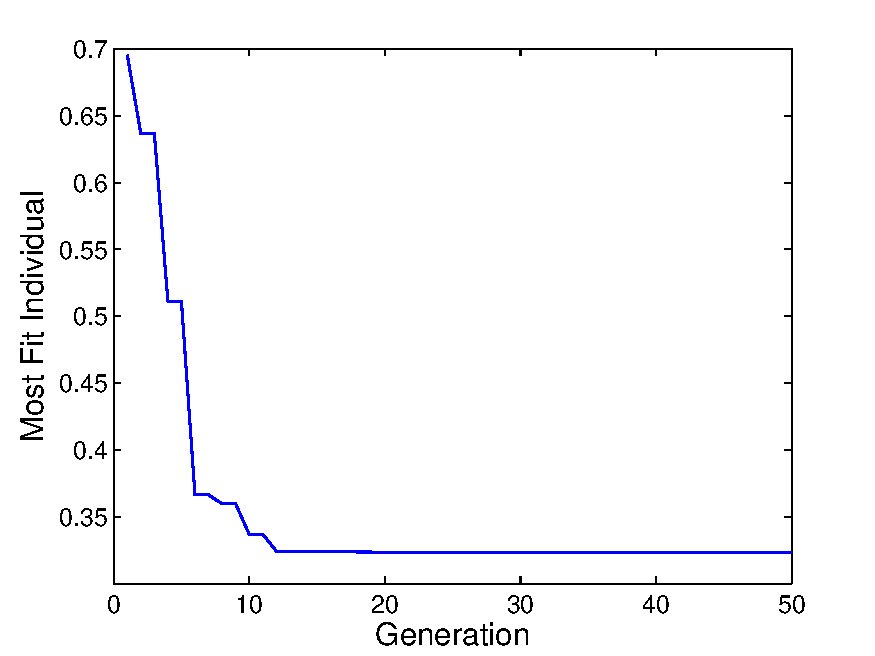
\includegraphics{images/popFitness.pdf}} \subfigure[Individual fitness average by
generation.\label{f:popaverage}]{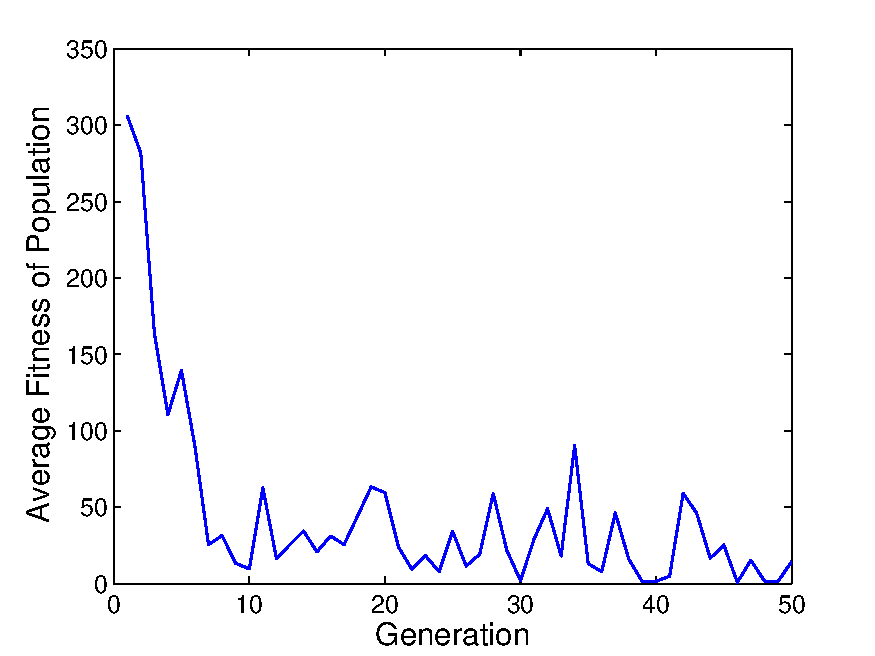
\includegraphics{images/popAverage.pdf}} \end{subfigmatrix} \end{figure}

\subsection{Genetic Adaptability} These results demonstrate the ability of the genetic algorithm to tune a FIS
to near-optimal performance. All tuning and development heretofore was done with an unchanging system setup of
known masses connected by a known spring. Although a robust controller\cite{cohen:01jgcd}, introducing changes
to the masses of each car significantly alters the performance of the FIS as it was carefully tuned to only a
certain envelope; however, utilizing the genetic algorithm to generate an optimum FIS for each new system
setup is an efficient method of developing good active controllers. This is demonstrated by changing the
masses $m_1$ and $m_2$ to \SI{2}{\kilogram} and \SI{4}{\kilogram} respectively. They are again changed to
\SI{4}{\kilogram} and \SI{8}{\kilogram}, and finally \SI{4}{\kilogram} and \SI{16}{\kilogram}. The algorithm
was deployed for each case to optimize a controller for that envelope. After fifty generations of evolution,
the genetically optimized FIS performed within 3\% of the theoretical rigid body limit in all four cases.
These results are displayed in \cref{tab:gacomp}.  \begin{table} \centering \caption{Genetic algorithm
    FIS performance compared the hand-tuned FIS and rigid body limit.} \label{tab:gacomp}
    \begin{tabular}{|c|c|c|c|c|} \cline{2-5} \multicolumn{1}{c|}{} & \multicolumn{4}{|c|}{Mass 1
        (\si{\kilogram}), Mass 2 (\si{\kilogram})} \\\cline{2-5} \multicolumn{1}{c|}{} & \SI{1}{\kilogram},
        \SI{2}{\kilogram} & \SI{2}{\kilogram}, \SI{4}{\kilogram} & \SI{4}{\kilogram}, \SI{8}{\kilogram} &
        \SI{4}{\kilogram}, \SI{16}{\kilogram} \\\hline Theoretical Limit & 0.3191 & 0.4553 & 0.6438 & 0.8312
        \\\hline GA FIS & 0.3231 & 0.4562 & 0.6579 & 0.8434 \\\hline Hand-tuned FIS & 0.3233 & 0.6125 & 5.3072
                        & 3.3240 \\\hline\hline GA Error & \multicolumn{1}{|d|}{1.3\%} &
        \multicolumn{1}{|d|}{0.2\%} & \multicolumn{1}{|d|}{2.2\%} & \multicolumn{1}{|d|}{1.5\%} \\\hline
        Hand-tuned Error & \multicolumn{1}{|d|}{1.3\%} & \multicolumn{1}{|d|}{34.5\%} &
        \multicolumn{1}{|d|}{724.4\%} & \multicolumn{1}{|d|}{299.9\%} \\\hline \end{tabular} \end{table}

It is easily seen in these results that the use of the genetic algorithm is advantageous in the autonomous
development of near optimal FIS controllers. Given a generic control architecture, the genetic algorithm is
able to tune a FIS rapidly and accurately for a varied set of circumstances.

\section{Conclusions} Fuzzy logic provides a robust framework for control. It has
been demonstrated that proper fuzzy control is efficient and computationally inexpensive. The inherent
vagueness of set membership and linguistic operation of fuzzy logic allows the controller to mimic expert
human control. This superior control, however, comes with a steep cost in FIS development. Hand-tuning a FIS
is time-consuming and tedious.


The use of the genetic algorithm facilitates FIS development. Once a FIS has been developed for a general type
of control situation, it is relatively simple to define the FIS as a genetic element and automate the tuning
through the evolutionary process. These results imply that if a general fuzzy controller is developed for a
family of control situations, then a genetic algorithm can be implemented to tune each FIS to its specific
task. The tuning, therefore, can be accomplished by someone with no expertise in the control of the situation.
As the computation is quick, efficient control could be widely distributed due also to the low-cost of
development.


